\section{Simulaciones}
\label{sc:rr_simulation}

Las simulaciones se realizaron sobre las herramientas Meep y Lumerical en 2 máquinas con
las siguientes características:

\begin{table}[H]
\centering
\begin{tabular}{|c|}
\hline
Procesador intel core i7 980X. Frecuencia de Reloj OC 4.5 GHz. \\
6 núcleos - 12 hilos. \\
24 GB de Memoria RAM a bus de 1600MHz. \\
GPU nVidia GTX580. \\
2 discos duros de estado solido de 128 GB en RAID 0. \\
\hline
\end{tabular}
\caption{Equipo para simulación en Lumerical. Codename: Amelie}
\label{tb:pcsim1}
\end{table} 

\begin{table}[H]
\centering
\begin{tabular}{|c|}
\hline
Procesador intel core i7 Ivy Bridge, 3770k. Frecuencia de reloj OC 4.4 GHz \\
4 núcleos - 8 hilos. \\
16 GB de RAM a bus de 1600 MHZ \\
GPU ATI 7950. ASUS DirectCU II \\
128 GB  de disco duro de estado sólido sata3 \\
\hline
\end{tabular}
\caption{Equipo para simulación en Meep. Codename: Arwen}
\label{tb:pcsim2}
\end{table} 

\subsection{Diseño del Resonador}
\label{sss:rr_design}

Para el diseño del simulador, se siguieron los lineamientos descritos en \cite{Lumerical2009}
tanto para el filtro AddDrop como para el filtro Notch. El primero consiste en
el modelo explicado en la sección \ref{ss:generic_theory} con la salvedad que 
la región de Acoplamiento 1 es idéntica a la región de Acoplamiento 2, por lo tanto
$\kappa = \kappa_1 = \kappa_2$, 
$\kappa^* = \kappa_1^* = \kappa_2^*$, 
$t=t_1 = t_2$ y 
$t^*=t_1^* = t_2^*$. 
Adicionalmente, se asume que no hay pérdidas $(\alpha=1)$ y
se seleccionan las características dadas en la tabla \ref{tb:lum_params}.

\begin{table}
\centering
\begin{tabular}{|l|l|}
\hline
Parámetro & Valor \\
\hline
Rango de frecuencias & 1500nm a 1600nm \\ 
$\lambda_0$ & 1550nm \\
Espaciamiento de canales & 200Ghz ó 1.6nm a 1550nm \\
$FSR$ & 3200GHz ó 25.6nm a 1550nm ó 16 canales \\
$\Delta \lambda_{FWHM}$ & 100GHz ó 0.8nm \\
$Q$ & $\frac{1550nm}{0.8nm} \approx 2000$  (\ref{eq:q})\\
\hline
\end{tabular}
\caption{Configuración deseada para el filtro}
\label{tb:lum_params}
\end{table} 

\subsubsection{Índice de grupo $n_g$}

Se calcula el índice de grupo $n_g$ mediante la herramienta MODE de lumérical
(seccion \ref{ss:lumerical}) para encontrar los valores propios en un rango de 
frecuencias de interés. En la gráfica \ref{fig:ng} se
ve el perfil del primer modo a la izquierda y la gráfica de longtud de onda
vs índice de grupo a la izquierda. A partir de ésta, se visualiza que para
$\lambda_0=1550nm$ se tiene $n_g\approx4.8$.

\begin{figure}[h!]
\caption{Índice de grupo. Fuente\cite{Lumerical2009}}
\centering
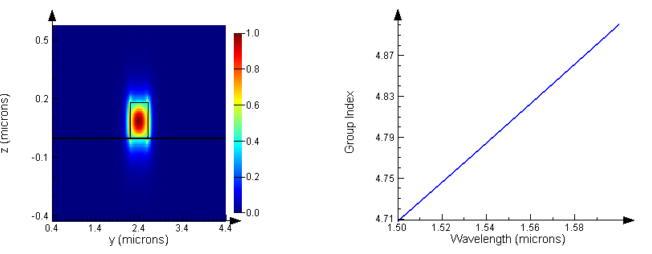
\includegraphics[width=0.8\textwidth,natwidth=652,natheight=254]{figs/ng.png}
\label{fig:ng}
\end{figure} 

\subsubsection{Perímetro del anillo}

Despejando $L$ partir de (\ref{eq:fsr}) y sustituyendo los parámetros 
(Tabla \ref{tb:lum_params}), se tiene:

\begin{align*}
L=\frac{\lambda_0^2}{n_g FSR} 
&=\frac{1550e-9}{4.8 \times 25.6e-9}
 =19.5 \mu m  \\ %\label{eq:lum_l} \\
R &= \frac{L}{2 \pi} = 3.1 \mu m  %\label{eq:lum_r}
\end{align*}

\subsubsection{Coeficiente de transmisión y acoplamiento} 

Al despejar $|t|$ de (\ref{eq:q}) se tiene:

\begin{equation}
|t|=\sqrt{ \left( \frac{n_g L \pi}{2 Q \lambda} \right) ^2 + 1} - 
    \frac{n_g L \pi}{2 Q \lambda}
\label{eq:t}
\end{equation} 

Y remplazando la configuración dada en la tabla \ref{tb:lum_params}:
\begin{equation*}
|t|=\sqrt{ \left( \frac{4.8 19.5e-6 \pi}{2 2000 1550e-9} \right) ^2 + 1} - 
    \frac{4.8 19.5e-6 \pi}{2 2000 \lambda}
   \approx 0.954
\label{eq:lum_t}
\end{equation*}

El valor de $\kappa$ se obtiene despejando (\ref{eq:energy_conserv}):

\begin{equation}
|\kappa|=\sqrt{1 - |t|^2} \approx 0.301
\label{eq:lum_k}
\end{equation} 

\subsubsection{Transmitancia}

De (\ref{eq:energy_conserv}) y (\ref{eq:T_d}) y teniendo en cuenta 
las consideraciones de la tabla \ref{tb:lum_params} se tiene:

\begin{align}
T_d&=\frac{|\kappa^4|}{|1 - t^2 e^{j \beta L}|^2} \label{eq:lum_Td} \\
T_t&=\frac{|t -t e^{-j \beta L}|^2}{|1 - t^2 e^{j \beta L}|^2} \label{eq:lum_Tt} 
\end{align} 

\subsection{Lumerical}

\subsubsection{Diseño del Resonador}
\label{sss:rr_design}

Para el diseño del simulador, se siguieron los lineamientos descritos en \cite{Lumerical2009}.
El espaciamiento de los canales será de 200GHz ó 1.6nm a 1550nm. Cada 16 canales,
la portadora resonará en el anillo, lo que indica un FRS de 3200GHz ó 25.6nm a 1550nm.
El ancho del pulso en la mitad de la potencia (FWHM) será de 100GHZ, es decir que
el factor de calidad (Q) es de aproximadamente 2000.

%TODO: Poner fórmulas



% The first argument is the script location/filename and the second is a caption for the listing
\subsection{Meep}
\label{ss:c1_meep}

Meep es un software desarrollado en el Massachusetts Institute of Technology - MIT
que implementa el método FDTD. 
Su nombre es un acrónimo que proviene de las iniciales de 
“MIT Electromagnetic Equation Propagation” y cuenta con las siguientes características 
\cite{oskooi2010meep}:

\begin{itemize}
\item Simulación 1D, 2D, 3D
\item Soporte MPI
\item Fronteras Absorción  PML 
\item Scripts  en Scheme (*.ctl)
\item Scripts en C++
\item Análisis de flujos, frec, energía ...
\item Licencia GNU/GPL
\end{itemize} 

\subsubsection{Filtro Notch}

El código está dividido en 5 secciones en cada una de las cuales se define: 
\begin{enumerate}
\item Parámetros de la simulación.
\item Materiales y geometría a simular.
\item Fuente de onda electromagnética.
\item Puntos de medición de flujo de energía.
\item Tiempos y salidas de la simulación.
\end{enumerate} 

A continuación, se explicará el objetivo y el contenido de cada subsección 
sólo del script para el filtro Notch. Para ver el script completo 2D y 3D
de los 2 filtros, ver el apéndice \ref{ap:meep}.

\subsubsection{Parámetros}
\zcodectl{"sources/c1_meep_s1.ctl"}{Parámetros Filtro Notch.} 
En esta sección de código (Script \ref{"sources/c1_meep_s1.ctl"}) 
se especifican los parámetros necesarios para la ejecución de los programas. 
Se usaron 2 tipos diferentes de instrucciones: $define$ y $define-param$. 
La primera instrucción, de la forma $(define <variable> <expresion>)$, es nativa de Scheme y permite 
ejecutar una expresión dada por medio de una variable. 

Por el contrario, $define-param$, está definida en una librería de extensión llamada LibCtl y permite que la 
asociación de la variable a la expresión sea modificada desde la línea de comandos desde la que se invoca el 
programa permitiendo tener un control flexible para las simulaciones. 

Los parámetros usados en la simulación del filtro están especificados en 
la Tabla \ref{tb:meep_params}.

\begin{table}[H]
\centering
\begin{tabular}{| l | l | c | }
\hline
Parámetro & Descripción & Valor x Defecto \\
\hline
$w$ &	Ancho de la guía de onda &  4 nm \\
$r$ &	Radio interno del anillo resonador &	2.9 $\mu$m \\
$gap$ &	Espacio entre la guía de onda y el anillo & 1 nm \\
$dpml$ &    Ancho de la capa PML &  2  $\mu$m \\
$wavecen$ & Ancho de banda central de la fuente &   1550 nm \\
$waveid$ &  Ancho del pulso de la fuente &  50 nm \\
$freqcen$ & Frecuencia central de la fuente &	$\frac{1}{wavecen}$ \\
$freq_width$ &	Ancho del pulso de la fuente (en frecuencia) &	$\frac{1}{wavecen-waveid} - \frac{1}{wavecen+waveid}$ \\
\hline
\end{tabular}
\caption{Parámetros}
\label{tb:meep_params}
\end{table}


\subsubsection{Materiales y Geometría}

En esta sección se emplearon algunos de los parámetros definidos en
la tabla \ref{tb:meep_params} para construir la geometría del filtro como se ve en
la figura \ref{fig:notch_geometry}.

\begin{figure}[H]
\caption{Geometría Filtro Notch.}
\centering
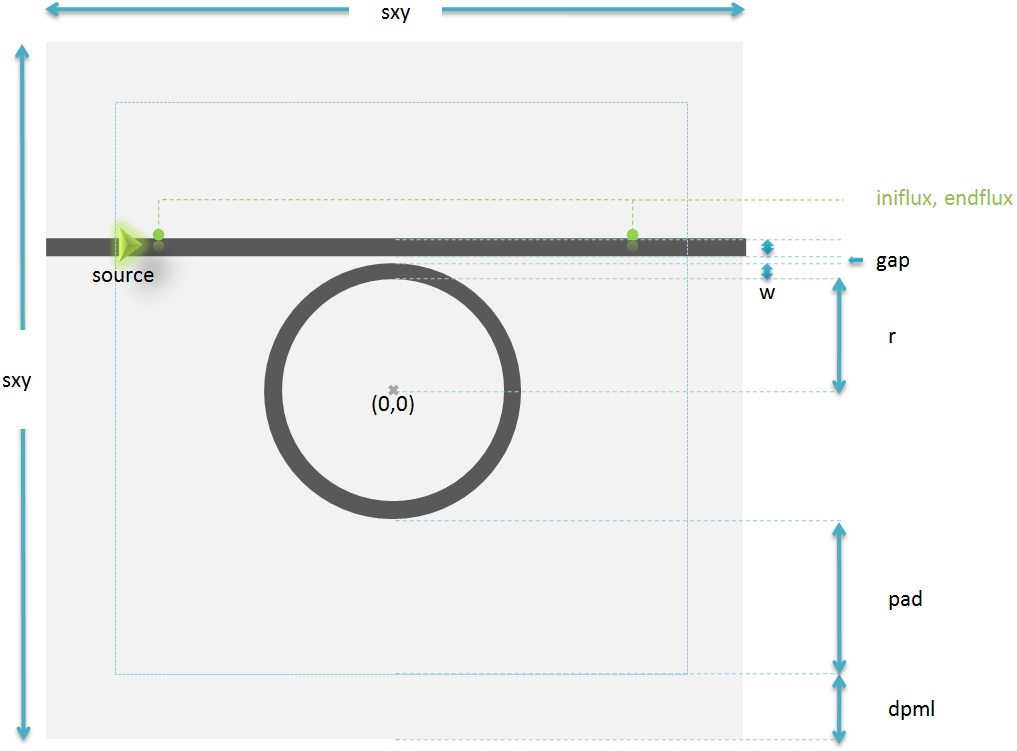
\includegraphics[width=1.0\textwidth,natwidth=892,natheight=663]{figs/notch_v2.jpg}
\label{fig:notch_geometry}
\end{figure}

Como se aconseja en \cite{MIT_tuto} 
el tamaño del látice a simular se calcula 
de forma dinámica a partir de los parámetros del radio, ancho de la guía de onda, 
espacio de holgura y el borde PML (Script \ref{"sources/c1_meep_s2.ctl"}). 

\zcodectl{"sources/c1_meep_s2.ctl"}{Geometría y Materiales Filtro Notch.} 
Silicon Photonics utiliza, como su nombre lo indica, silicio como medio para la propagación de ondas electromagnéticas en el espectro C-Band . 
Por lo tanto, para la longitud de onda de 1500 nm, el índice de refracción del silicio corresponde a 3.4765 \cite{bass2009handbook}. 
Adicionalmente, al ser una simulación en 2D, el material que rodea la guía recta y circular es el aire cuyo índice de refracción es 1. 
La base de dioxido de silicio SiO2 sobre la cual está montada la guía, sólo se tomó en cuenta para la simulación 3D (sección \ref{ss:lumerical}).

%TODO Preguntarle a jose: http://ab-initio.mit.edu/wiki/index.php/Meep_Tutorial 
%Thus, 0.15 corresponds to a vacuum wavelength of about 1 / 0.15 = 6.67, or a wavelength of about 2 in the  material—thus, our waveguide is half a wavelength wide, which should hopefully make it single-mode. (In fact, the cutoff for single-mode behavior in this waveguide is analytically solvable, and corresponds to a frequency of 1/2√11 or roughly 0.15076.)

La guía de onda se especifica como un rectángulo de Si, mientras que la estructura del anillo se construye a partir de la superposición de un cilindro externo de silicio y un cilindro interno de aire. 
Las dos estructuras están separadas en su punto más cercano por una distancia 
definida por el parámetro $gap = 100nm$.

Finalmente, se indicó una resolución de 
%TODO Resolución%

\subsubsection{Fuente de Onda Electromagnética} 
Como se mencionó anteriormente, una de las aplicaciones de FDTD es el cálculo 
de la transmisión o la dispersión del espectro de estructuras tales como cavidades 
resonantes en respuesta a un estímulo de entrada. Una forma de obtener estos 
datos es calcular el flujo transmitido para cada frecuencia $\omega$ de forma 
separada. Una forma más rápida es calcular la respuesta a un conjunto 
amplio de espectros usando un sólo cálculo de la transformada de Fourier usando un 
pulso gaussiano de banda ancha \cite{MIT_intro}. 

En este trabajo se simularon estas 2 formas (cada una en un script diferente)
tanto para el filtro Notch, como para el filtro AddDrop.


\subsubsection{Resultados}

\begin{figure}[H]
\caption{Transmitancia Filtro Notch}
\centering
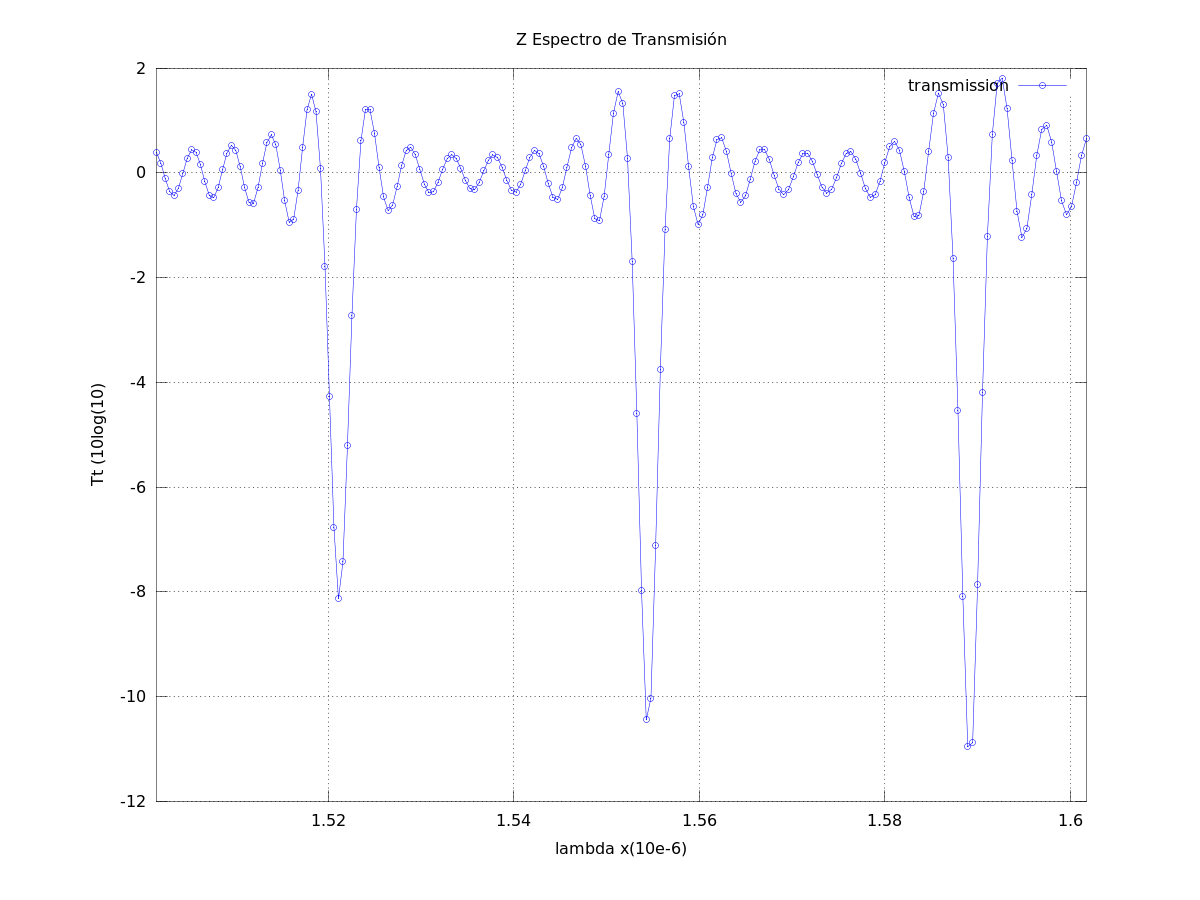
\includegraphics[width=1.0\textwidth,natwidth=1200,natheight=900]{figs/gausrc_flux_mod-graph_res80.png}
\label{fig:meep_res_n}
\end{figure}

\begin{figure}[H]
\caption{Filtro Notch 3d vista [X,Y], [Y,Z] y [X,Z] respectivamente. (a)(b)(c) Material Dieléctrico. (d)(e)(g) Campo eléctrico $E_z$ }
\centering
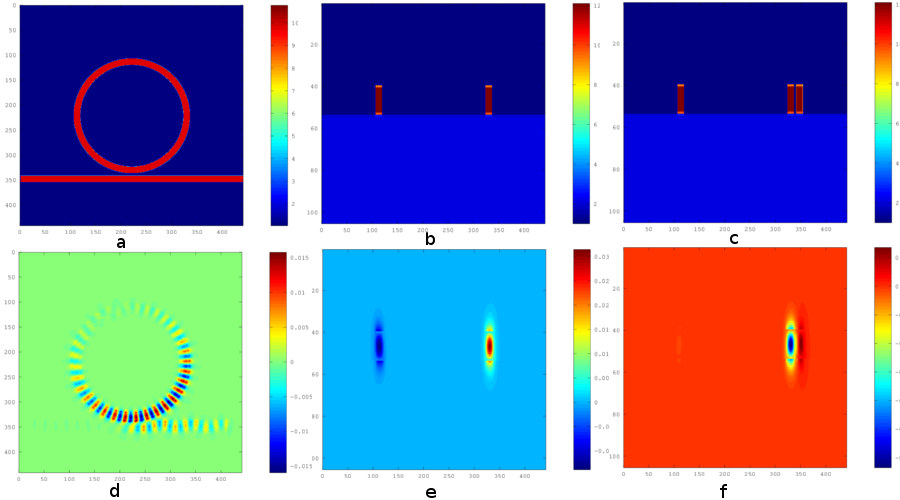
\includegraphics[width=1.0\textwidth,natwidth=900,natheight=500]{figs/notch3d.png}
\label{fig:notch_geometry}
\end{figure}

\begin{figure}[H]
\caption{Transmitancia Filtro Notch 3D}
\centering
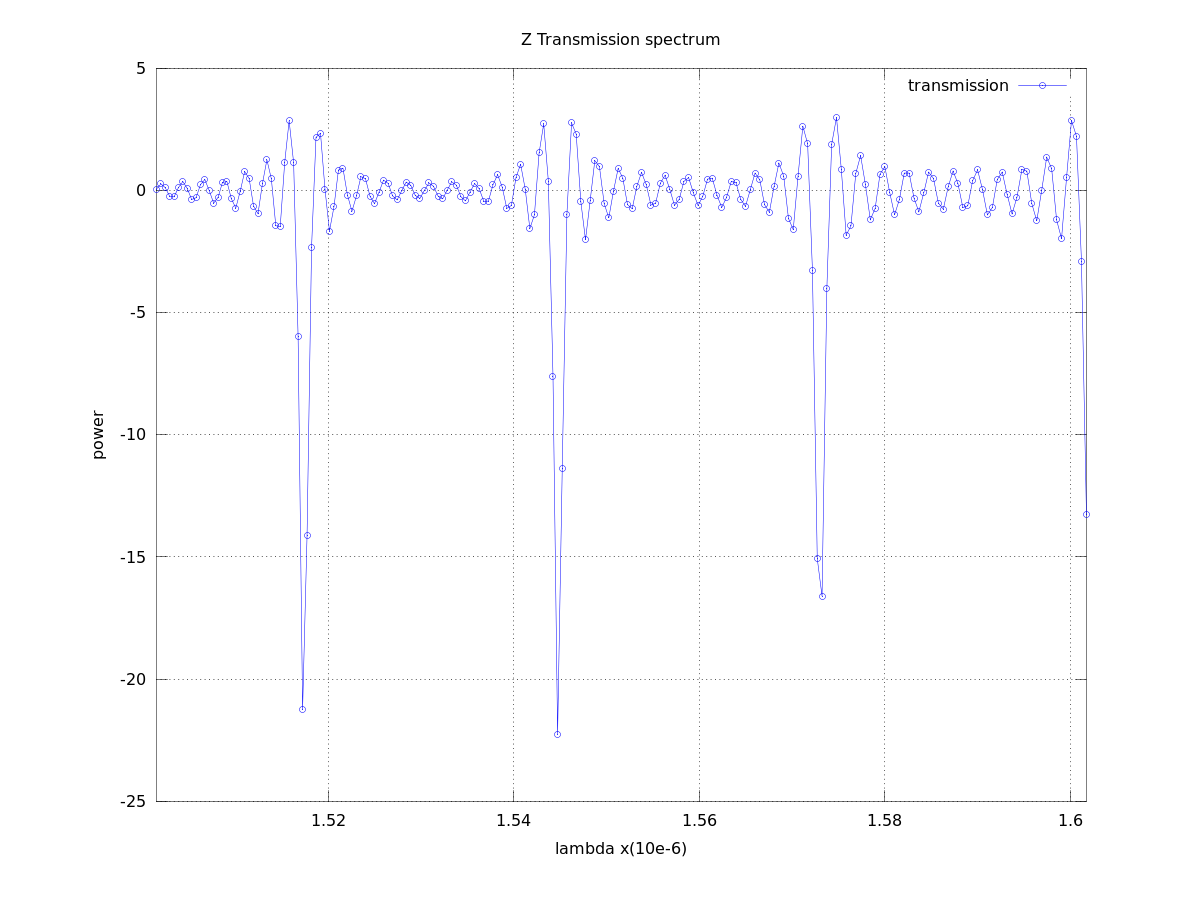
\includegraphics[width=1.0\textwidth,natwidth=1200,natheight=900]{figs/notch3d_T.png}
\label{fig:meep_res_n}
\end{figure}


Se pueden observar diferencias en cuanto al valor teórico esperado en las
condiciones de resonancia para todas las simulaciones,
debido a que se asumió que el anillo no presentaba pérdidas $(\alpha = 1)$ en
el cálculo teórico de la transmitancia.

Sin embargo, la que más difiere de todas inclusive en el FSR esperado 
es la simulación mostrada en la figura \ref{fig:meep_res_n}. Esto se puede deber a
que esta simulación se realizó sólamente en 2 dimensiones y por lo tanto
deja de lado la interacción de la onda con el materia de Sílica SiO2.


\subsection{Conclusiones y Trabajos Futuros}
\begin{itemize}
\item Las frecuencias de resonancia del anillo pueden ser manipuladas mediante
modificaciones en el diámetro del anillo, el gap o el índice de refracción. Este
último es de gran importancia por ser la base del funcionamiento algunos dispositivos
moduladores en Silicon Photonics donde se aplica un campo
magnético, generando un efecto plasmónico que altera el índice y por lo tanto
los modos de resonancia.
\item Debido a que se asumió que el anillo no presentaba pérdidas $(\alpha = 1)$ en
el cálculo teórico de la transmitancia tanto del filtro Notch como del filtro
AddDrop, se pueden apreciar diferencias en las condiciones de resonancia
de la teoría con respecto a lo obtenido en la práctica.
\item Las diferencias en el $FSR$ obtenido en las simulaciones realizadas en Meep
con respecto a las realizadas en Lumerical, pueden ser explicadas debido a la 
diferencia en las dimensiones de ambas simulaciones. Mientras que en Lumerical 
se realizó una simulación 3D de ambos filtros, en Meep la mayoría fueron realizadas
en 2D a diferencia del último caso. Este escenario permitió corroborar esta teoría
ya que la simulación Meep 3D del filtro Notch fue muy similar a la simulación del mismo
filtro en la plataforma Lumerical.
\item Como trabajo futuro se plantea realizar nuevas simulaciones para los dos
filtros modificando el diámetro del anillo para visualizar 
la alteración en el FSR y su uso como filtro selectivo o filtro de banda ancha.
\item Se propone también, para un diámetro fijo, realizar simulaciones alterando 
el índice de refracción del anillo para simular el efecto plasmónico que 
sucede dentro del modulador y que hace que se desplacen las frecuencias de resonancia
de un estado On a Off.
\end{itemize} 

